\documentclass{article}
\usepackage[spanish]{babel} %Definir idioma español
\usepackage[utf8]{inputenc} %Codificacion utf-8
\usepackage{amssymb, amsmath, amsbsy, wasysym}
\usepackage{multirow} % para tablas
\usepackage{graphicx}
\usepackage[dvipsnames]{xcolor}
\title{Práctica 3}
\author{Emmanuel Peto Gutiérrez}
\begin{document}
\maketitle

\section{Introducción}

Esta práctica consiste en implementar los siguientes algoritmos de búsqueda:

\begin{itemize}

\item[1.] Búsqueda Secuencial

\item[2.] Búsqueda Binaria

\item[3.] Búsqueda Exponencial

\item[4.] Búsqueda por Interpolación

\end{itemize}

\section{Descripción}

\subsection{Entrada}

El programa a implementar debe recibir como entrada en los argumentos de la linea de comandos:

\begin{itemize}
\item[1.] Nombre del archivo de texto que contiene los elementos del espacio de
búsqueda (Números separados por ` ').
\item[2.] Elemento a buscar(un único número entero).
\item[3.] Algoritmo a utilizar para la búsqueda. (Especificar en el readme cómo se indica al programa el algoritmo a utilizar)
\end{itemize}

Por ejemplo, utilizando Búsqueda Lineal sobre el archivo ``Numeritos.txt'' para encontrar el número 7:

\begin{center}
java Search Numeritos.txt 7 lineal
\end{center}

\subsection{Formato}

El archivo de texto de entrada contendrá la información necesaria para definir
el espacio de búsqueda. Esto es:

-Una o más lineas, con los números de entrada separados por ` '(espacio).

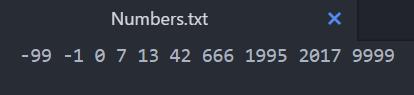
\includegraphics[scale=0.5]{entrada}

\subsection{Salida}

La salida del programa será por medio de terminal y debe mostrarse el índice del elemento buscado en el espacio de búsqueda especificado. En otro caso, el programa debe indicar si el elemento no se encuentra en el espacio de búsqueda.

\section{Detalles}

La práctica debe ser implementada utilizando Java.

\subsection{Extra}

Para obtener calificación adicional en esta práctica se debe anexar un método
para generar listas ordenadas(como los archivos de entrada). El método generador de secuencias ordenadas no debe ser trivial, se tomará en cuenta principalmente qué tan creativo e ingenioso es, y su funcionamiento debe ser explicado ya sea en el Readme o en la documentación del código.


\section{Entrega}

\begin{itemize}
\item Deben entregarlo como un archivo comprimido de una carpeta con el mismo nombre.
\item La carpeta debe ser: \textbf{Practica3\_ApellidopaternoApellidomaterno}. Por ejemplo \textbf{Practica3\_PetoGutierrez}.
\item Su carpeta debe contener un archivo \emph{readme} que contenga: número de cuenta, nombre completo, 
correo y las instrucciones para compilar y ejecutar su programa(se recomienda un \emph{Makefile}).
\item Si su carpeta contiene un ejecutable(como *.jar) enviarlo como un enlace de dropbox o drive.
\item El asunto debe ser: \textbf{[AAlgoritmos]Practica3}.
\item El correo al que enviarán la práctica es: \emph{empg014@ciencias.unam.mx}
\end{itemize}

La fecha de entrega de esta práctica será el martes \textbf{1 de octubre}.

\end{document}

